\documentclass[sigconf,table,screen,xcdraw,review]{acmart}

\usepackage{booktabs} 
\usepackage{framed}
\usepackage{graphicx}
\usepackage{subfigure}
\usepackage{pifont}
\usepackage{xspace}
\usepackage{multirow}
\usepackage{xcolor,colortbl}
\usepackage{hhline}
\usepackage{adjustbox}
\usepackage{booktabs} 
\usepackage{amssymb}
\usepackage{balance}
\usepackage{tcolorbox}
\usepackage{url}
\usepackage{booktabs}
\usepackage{paralist}
\usepackage{enumitem}
\usepackage{lipsum}
\usepackage{listings}
\usepackage{tikz}
\usepackage{pgfplots}
\usepackage{amssymb}
\usepackage{standalone}
\usepackage{url}

\usepackage[ruled,vlined,linesnumbered]{algorithm2e}
\definecolor{codegreen}{rgb}{0,0.6,0}
\definecolor{codegray}{rgb}{0.73,0.38,0.06}
\definecolor{codepurple}{rgb}{0.27,0.38,0.97}
\definecolor{codemagenta}{rgb}{0.74,0.09,0.42}
\definecolor{backcolour}{rgb}{0.96,0.96,0.96}

% for footnotes on the same line
\usepackage[para]{footmisc}
\setcitestyle{numbers,sort&compress}

\newcommand\iris{\textsc{DisDrillery}\xspace}

\newcommand*{\ColorIfNotInString}[1]{\color{codegray}\textbf{#1}}%

\lstdefinestyle{mystyle}{
    backgroundcolor=\color{backcolour},   
    commentstyle=\color{codegreen},
    keywordstyle=\color{codepurple},
    numberstyle=\tiny\color{codegray},
    stringstyle=\color{codemagenta},
    language=Java,
    breakatwhitespace=false,         
    breaklines=true,                 
    keepspaces=true,                 
    numbers=left,
    xleftmargin=0.25cm,                    
    numbersep=5pt,                  
    showspaces=false,                
    showstringspaces=false,
    showtabs=false,                  
    tabsize=1,
    frame=tb,
    framerule=0pt,
    literate=%
    {0}{{{\ColorIfNotInString{0}}}}1
    {1}{{{\ColorIfNotInString{1}}}}1
    {2}{{{\ColorIfNotInString{2}}}}1
    {3}{{{\ColorIfNotInString{3}}}}1
    {4}{{{\ColorIfNotInString{4}}}}1
    {5}{{{\ColorIfNotInString{5}}}}1
    {6}{{{\ColorIfNotInString{6}}}}1
    {7}{{{\ColorIfNotInString{7}}}}1
    {8}{{{\ColorIfNotInString{8}}}}1
    {9}{{{\ColorIfNotInString{9}}}}1
}
% \usepackage{inconsolata}
\lstset{basicstyle=\fontsize{6}{6}\fontfamily{\ttdefault}\selectfont,style=mystyle}

\renewcommand{\arraystretch}{1.2}

\usepackage{hyperref}
\usepackage{cleveref}

\newcommand{\todo}[1]{{\color{red}TODO: #1}}
\newcommand{\citeTodo}[1]{{\color{red}[??]}}
\newcommand{\checkNum}[1]{{\color{black}$#1$}}
\newcommand{\ie}{\emph{i.e.},\xspace}
\newcommand{\Ie}{\emph{I.e.},\xspace}
\newcommand{\eg}{\emph{e.g.},\xspace}
\newcommand{\Eg}{\emph{E.g.},\xspace}
\newcommand{\etal}{\emph{et al.}\xspace}

\setlength{\floatsep}{2pt}
\setlength{\textfloatsep}{5pt}

\newcommand*\circled[1]{\tikz[baseline=(char.base)]{
    \node[shape=circle,draw,inner sep=0.5pt] (char) {#1};}}

\newenvironment{myquote}{\list{}{\leftmargin=0.08in\rightmargin=0.08in}\item[]}{\endlist}

{\newcommand{\nb}[2]{
    \fbox{\bfseries\sffamily\scriptsize#1}
    {\sf\small$\blacktriangleright$\textit{#2}$\blacktriangleleft$}
  }
\renewcommand{\arraystretch}{1.2} 
\newcommand\GIOVANNI[1]{\nb{\textcolor{red}{Gio}}{\textcolor{red}{#1}}}
\newcommand\FABIO[1]{\nb{\textcolor{red}{Fabio}}{\textcolor{red}{#1}}}
\newcommand\FABIANO[1]{\nb{\textcolor{red}{Fabiano}}{\textcolor{red}{#1}}}
\newcommand\ANDREA[1]{\nb{\textcolor{red}{Andrea}}{\textcolor{red}{#1}}}
\newcommand\HCG[1]{\nb{\textcolor{red}{Harald}}{\textcolor{red}{#1}}}

\newcommand\RQ[1]{\textbf{RQ$_#1$}}

\definecolor{gray50}{gray}{.5}
\definecolor{gray40}{gray}{.6}
\definecolor{gray30}{gray}{.7}
\definecolor{gray20}{gray}{.8}
\definecolor{gray10}{gray}{.9}
\definecolor{gray05}{gray}{.95}

\newlength\Linewidth
\def\findlength{\setlength\Linewidth\linewidth
  \addtolength\Linewidth{-4\fboxrule}
  \addtolength\Linewidth{-3\fboxsep}
}
\newenvironment{examplebox}{\par\begingroup
  \setlength{\fboxsep}{5pt}\findlength
  \setbox0=\vbox\bgroup\noindent
  \hsize=0.95\linewidth
  \begin{minipage}{0.95\linewidth}\normalsize}
  {\end{minipage}\egroup
  %    \vspace{6pt}
  \textcolor{gray20}{\fboxsep1.5pt\fbox
    {\fboxsep5pt\colorbox{gray05}{\normalcolor\box0}}}
  %    \endgroup\par\addvspace{6pt minus 3pt}\noindent
  \endgroup\par\noindent
  \normalcolor\ignorespacesafterend}
\let\Examplebox\examplebox
\let\endExamplebox\endexamplebox


\newenvironment{resultbox}{\par\begingroup
  \setlength{\fboxsep}{5pt}\findlength
  \setbox0=\vbox\bgroup\noindent
  \hsize=0.95\linewidth
  \begin{minipage}{0.95\linewidth}\normalsize}
  {\end{minipage}\egroup
  %    \vspace{6pt}
  \textcolor{gray20}{\fboxsep1.5pt\fbox
    {\fboxsep5pt\colorbox{white}{\normalcolor\box0}}}
  %    \endgroup\par\addvspace{6pt minus 3pt}\noindent
  \endgroup\par\noindent
  \normalcolor\ignorespacesafterend}
\let\Examplebox\examplebox
\let\endExamplebox\endexamplebox

\acmConference[MaLTeSQuE 2020]{MaLTeSQuE 2020: International Workshop on Machine Learning Techniques for Software Quality Evaluation}{November 13, 2020}{Sacramento, USA}
\acmBooktitle{MaLTeSQuE 2020: International Workshop on Machine Learning Techniques for Software Quality Evaluation, November 13, 2020 - Sacramento, USA}
\acmPrice{15.00}
\acmISBN{978-1-4503-9999-9/18/06}

\sloppy

\begin{document}

\title[Speeding Up the Data Extraction of Machine Learning Approaches]{Speeding Up the Data Extraction of Machine Learning Approaches: A Distributed Framework}
% \iris stays for d\textbf{I}st\textbf{R}ibuted m\textbf{I}ning \textbf{S}oftware repositories

	\author{Martin Steinhauer}
	\affiliation{%
		\institution{SeSa Lab - University of Salerno}
		\city{Fisciano (Salerno)}
		\state{Italy}
	}
	\email{m.steinhauer@studenti.unisa.it}

	\author{Fabio Palomba}
	\affiliation{%
	\institution{SeSa Lab - University of Salerno}
	\city{Fisciano (Salerno)}
	\state{Italy}
	}
	\email{fpalomba@unisa.it}

\begin{abstract}
In the last decade, mining software repositories (MSR) has become one of the most important sources to feed machine learning models. Especially open-source projects on platforms like GitHub are providing a tremendous amount of data and make them easily accessible. Nevertheless, there is still is a lack of standardized pipelines to extract data in an automated and fast way. Even though several frameworks and tools exist which can fulfill specific tasks or parts of the data extraction process, none of them allow neither building an automated mining pipeline nor the possibility for full parallelization. As a consequence, researchers interested in using mining software repositories to feed machine learning models are often forced to re-implement commonly used tasks leading to additional development time and libraries may not be integrated optimally. 

This preliminary study aims to demonstrate current limitations of existing tools and Git itself which are threatening the prospects of standardization and parallelization. We also introduce the multi-dimensionality aspects of a Git repository and how they affect the computation time. Finally, as a proof of concept, we define an exemplary pipeline for predicting refactoring operations, assessing its performance. Finally, we discuss the limitations of the pipeline and further optimizations to be done.\end{abstract}

\keywords{Machine Learning Pipelines; Distributed Mining; Mining Software Repositories.}
\maketitle


\section{Introduction}
\label{sec:intro}
The success of machine learning heavily relies on the amount and quality of data the algorithm is trained on. This is true not only for analyzing source code repositories but all learning strategies in general. At the the same time, the generation and extraction of suitable data is often based on a manual process which is costly and time-consuming. While getting the data for other machine learning settings is often difficult, the process of mining software repositories benefits from GitHub as one of the most important data sources and therefore has a high ability to be automated. The availability of GitHub data through big and public available open-source projects is one of the key aspects in MSR. Automation not only decreases the time spent on building datasets, it also improves the reproducibility of research projects and reusability of mining fragments throughout different projects when designed with generalization in mind.

However, in this preliminary work we show that the level of automation can be extended and improved by building a pipeline for automated repository mining and also improve the computation performance by applying a distributed parallelization approach already renowned in the area of big data processing. An exemplary pipeline is built that is able to detect and extract refactoring operations directly from GitHub repositories and calculates software quality metrics before and after the refactoring operation has been conducted. Eventually,  granular performance data is collected and evaluated to affirm the potential of further improvement and work.


\section{Background, Related Work, and Limitations of the State of the Art}
\label{sec:background}
\subsection{Related Work}
Previous research shows that there is a lack of reproducibility in most git-based research projects \cite{Robles2010}. Since then, some new frameworks and libraries evolved targeting the traversal of Git projects.\\
Common used frameworks to analyze the commit history of software repositories are RepoDriller \cite{repodriller} and PyDriller \cite{pydriller,Spadini2018}. Whereas both tools simplify the traversing of Git commits, PyDriller is able to calculate some basic metrics like complexity and method count. The metric calculation is done within the library and could not easily be replaced with custom metric logic. Additionally, PyDriller states to be multithreaded and therefore improve the performance and lower the calculation time. A closer look into the library shows that this statement is only partially true: PyDriller is based on the library GitPython which is restricted by visiting only one commit at a time. This is caused by the underlying file-based Git archive that enables thread-safety by locking the files during e.g. check out operations. Hence it is only possible to parallelize the processing in the file dimension but not in the time dimension (the commit history). In other words, only the iteration over files within one commit and then checkout the next commit which can be parallelized. The same theory applied to RepoDriller which relies on the Java-based alternative JGit \cite{jgit}. And besides, both tools allow no multi-repository mining and require additional orchestration and process management.\\
Other projects trying to avoid direct file system access and transferring repositories in an additional database before the first analysis. One well-known project is the GHTorrent project \cite{Gousios2012, Gousios2015} which allows various file-independent queries after importing the repository into a MySQL or MongoDB database. Unfortunately, the file content is not considered within this approach and only tooling for generating and importing is covered by them. \\
The project 'Public git archive' was introduced by researchers at sourced and allows us to analyze repositories from GitHub at a very large scale. They provide a lot of tools written in Go to query and also introduce a new storage format called Siva to reduce the stored size of forked repositories. Through a publicly available index file no additional processing is needed for developers. After the company was sold, the public available index file was taken down due to high costs and apparently was lost completely \cite{srcdissue}.

\subsection{Reproducibility challenge}
Related work shows that reprodicibility of the mining pipeline is a key feature to enable other researchers an easy reproduction and verification of the used dataset. Therefore, hosted datasets can become a nightmare since they require additional (financial) resources of the project holder and also are dependent on the life cycle of the initial project. If the project gets deprecated, all data could be gone like in the case of sourced. Mining data directly from GitHub may not resolve the problem of deleted or switched to private repositories and also introduce some overhead in terms of cloning and preprocessing but decreases the dependence to a hosting company or the creator of the project. Consequently, we will focus on the raw Git archive as a source of data.

\subsection{Multi-dimensionality of Git data}
At first glance, a GitHub repository looks like a tree-like timeline which contains different revisions and file versions along that axes. But from an algorithmic perspective, that can rapidly become an issue in terms of performance as every axis results in an iteration loop to reach at least each file once. This could also be described as multi-dimensionality of the Git data, as each additional dimension added to the mining process, will result more computation time and without considering the actual computation cost for detecting refactorings or calculating software quality metrics. Depending on the mining problem, we identified the following dimensions:\\
\begin{itemize}
    \item{\textbf{Time dimension:} Time dimension describes the total size of the analyzed commits. Git normally consists of one or more branches containing one main branch, denoted as \emph{master}. When traversing over the master branch, one will get all branches that have been merged into the master. In our case, we assume that for refactoring detection it would be sufficient to detect all valuable refactorings that have been considered as useful by merging them back into the master branch. Therefore, the time dimension of the refactoring detection could be seen as linear. When an analysis problem requires visiting every commit in the repository, the time dimension is considered as the total count of commits within the whole repository. }
    \item{\textbf{File dimension:} Defined by the file count one commit has in total. This amount of files can vary significantly and often depend on the project size, age of the project or the used programming language. Additionally, it is important to note that the file dimension is different for each commit as a file can be added or deleted within a commit. If the latest commits has only a few files and all others have many, the file dimension will affect the performance more as if the last commit have many files and the others have only a few. }
    \item{\textbf{Structural node dimension:} Similar to the file dimension, the total number of interesting nodes, for example, classes, methods or code lines, are counted in the content of each file. Considering object-oriented languages, a file normally contains one class, but also could consist of more than one class declaration. If the mining problem is dependent on method or class member declarations, those would also be considered as a number of interesting nodes per file.}
    \item{\textbf{Metric dimension:} The last dimension is very specific particularly regarding the mining problem. In our example, be would like to extract refactoring operations and calculate software quality metrics. Therefore, the metric dimension is highly coupled with the structural node dimension and defined by the method the metric is collected. RefactoringMiner \cite{Tsantalis:ICSE:2018:RefactoringMiner}} uses an abstract UML algorithm to detect refactorings, while CK \cite{aniche-ck} is using an abstract syntax tree (AST). Those algorithms also add on top of the file or structural dimension, depending on how they are implemented and designed.
\end{itemize}

\subsection{Parallelization challenge}
One of the biggest challenges is building a mining tool, that allows scaling of the mining process along the presented dimensionality axes. Both presented tools, PyDriller and RepoDriller, do not or only partially support the parallelization. While RepoDriller does not do any kind of parallelization, PyDriller allows scaling along the file dimension axis. Files within a single commit can be analyzed by multiple threads and increase the performance and decrease the computation time as the use of those libraries shows \cite{Gote2019}. As the multi-dimensionality of GitHub repositories outlines, we can not presume that repositories contain many files. When a repository contains fewer files but has a large revision history, the runtime of the mining process will get worse.\\
As already explained, the structural node dimension and the metric dimension are highly dependent on the type of analysis that should be executed. To make this approach generalizable, we focus on parallelization along the time and file dimension axes. As seen in PyDriller, the file dimension can easily be parallelized. In opposite, the commit axis is rather difficult: Since Git writes lock files when accessing the repository to avoid file inconsistencies by modifying the repository, only one commit can be visited concurrently. This limitation reflects in JGit and GitPython, which has all file-based actions marked as non-threadsafe. This limitation results in libraries not implementing a time dimension parallelization approach.

\subsection{Generalization challenge}
Even though we are conducting this distributed approach in the context of detecting refactoring operations, it is designed to be generalizable and can be reused for other types of mining problems. Since mining problems can vary from detecting developer behavior \cite{}, social aspects \cite{} up to high technical questions like code evolution \cite{} and smell detection\cite{}, it is not easy to build a pipeline that matches all type of problems. Therefore, this pipeline concentrates on technical, content-based repository mining.\\
Additionally, libraries are not standardized in their input and output design. While RefactoringMiner takes the repository and commits as an input, CK is designed not designed Git-specific and takes just the source directory as an input. This requires the pipeline to adopt the corresponding libraries in terms of in- and outputs of each pipeline step and even more important to keep track of the memory usage, since the libraries itself write outputs to disk, while within a pipeline, results sometimes are stored in memory. This causes a very careful design to avoid out of memory exceptions.

\section{\iris: A Distributed Framework to Support Machine Learning Research}
\label{sec:approach}

This section presents a distributed approach to support the data extraction process of machine learning approaches. For the sake of understandability, in the remaining of the paper we use the example of learning software metrics to predict the effect of refactoring operations on code quality: specifically, the example problem consists of computing software quality metrics before and after each refactoring applied on a certain system in order to assess the extent to which the refactoring has impacted on the values of those metrics. It is important to know, however, that the distributed approach proposed in this paper is general in scope, meaning that it can be exploited for any kind of data extraction activities related to the mining of software repositories. 

We are using a MapReduce-inspired pattern for data distribution and Apache Spark for pipeline implementation. MapReduce was originally invented by Google and targets big data analysis and calculations by splitting the computation process into a map and a reduce phase \cite{mapreduce2008} on a cluster of computation nodes. Those concepts are reimplemented and available as open source software in Apache Hadoop \cite{hadoop}. Spark improves this pattern by introducing resilient distributed datasets (RDDs) which are kept mainly in memory, which results in a faster processing speed than the traditional, hard-drive storage based Hadoop system. Also, Spark allows a better fault tolerance due to directed acyclic graphs (DAGs) for computation tasks. In case one task in the graph fails, Spark can easily restart that specific task without canceling the whole computation.

\begin{figure}
\caption{Overview of the refactoring mining pipeline.}
\centering
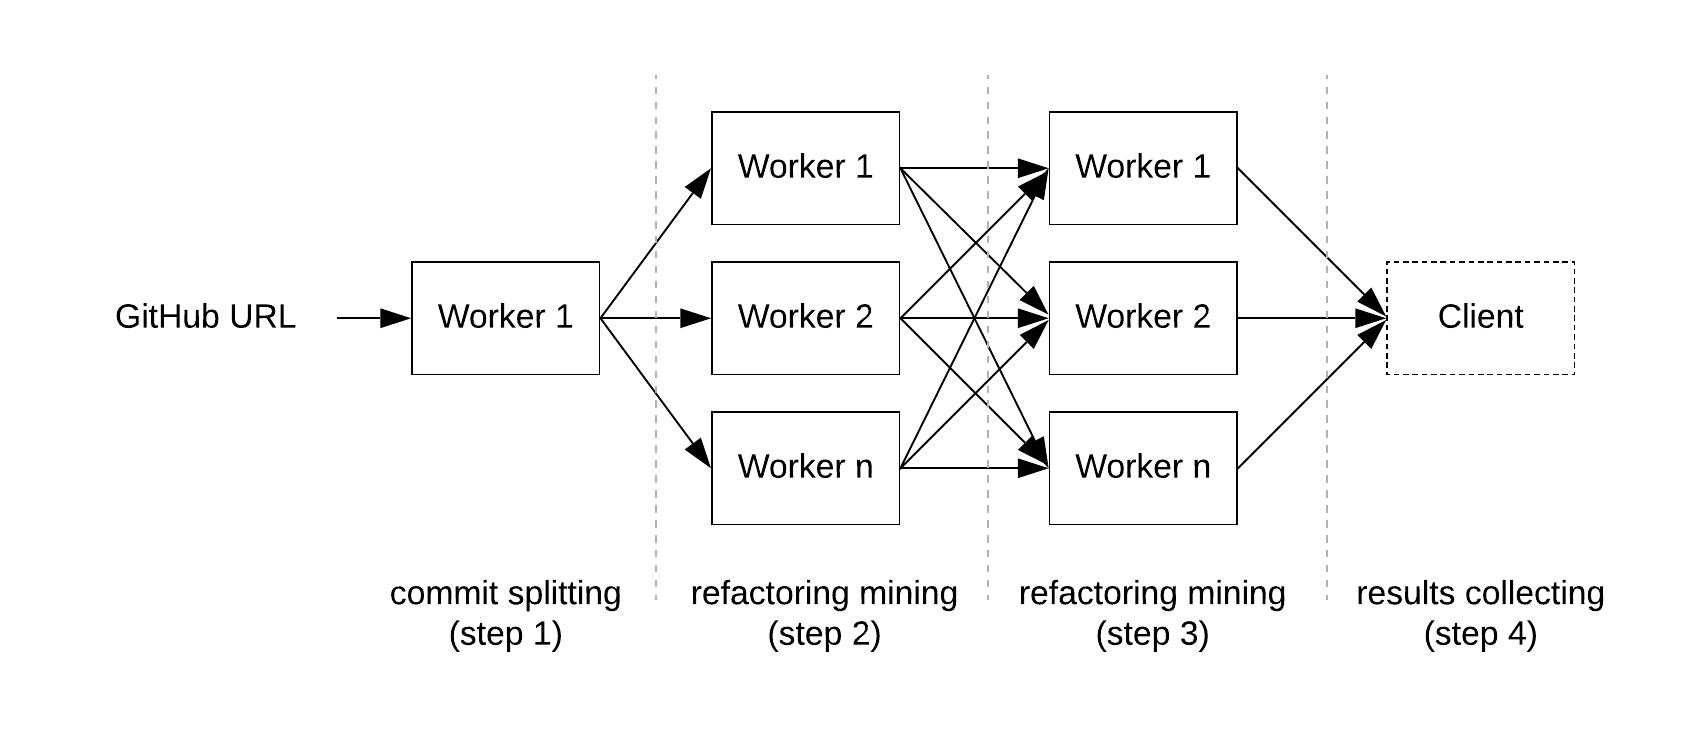
\includegraphics[scale=0.6]{pipeline}
\end{figure}

The pipeline is basically split into three major computation steps: The first step extracts the refactoring operations from a list of given repositories. Spark is cloning one repository instance and scans for commits along the master branch. The list of interesting commits is split into batches of a definable size of \emph{k}-commit and sent by shuffling to each of the other worker nodes.

In the second step, each worker starts cloning a separate instance of the repository if does not already exist and runs an instance of RefactoringMiner on the partial list of commits each worker has assigned. The previously described number of \emph{k}-commits depends on the size of memory each worker node has available, as the results are kept in the heap until one batch has finished the computation. Therefore, it is important to adjust \emph{k} accordingly: Is \emph{k} set too high, Spark will fail caused by out of memory exception. Is \emph{k} too small, the performance will decrease as instantiating an instance of RefactoringMiner is an expensive operation. This step outputs a list where each row consists of the repository name, the commit id of the refactoring operation and the type of the refactoring operation (e.g. move method, extract method...). The intermediate results are written as structured data using the Apache Parquet file format \cite{parquet} to reduce storage size and improve performance.

The third step takes the shuffled list of refactoring commits identified in the second step and starts again with checking if the repository exists. If not, it gets cloned to that worker node. Now for every batch of refactoring commits an instance of CK is created and the parent commit of the given commit is identified. After that, both commits are checked out and CK calculates the metrics before and after the commit. Additionally, to reduce the computation time and avoid useless data processing, those files that are marked as changed are identified by the Git diff command and the metric calculation is only executed for that list of modified files. As a result, another parquet file is generated containing information about the repository, the involved commits, the refactoring operations (flattened by comma separation), the \emph{side} of the operation (left = commit before refactoring, right = commit after refactoring), the file name, and the metrics.

\subsection{Implementation details}
Both libraries have not been very suitable to fit into our defined input and output format. Therefore they have been forked and slightly modified. RefactoringMiner only provides a method to detect a range of refactoring operations between two commit ids, though it found under certain circumstances more commits than actually existed in this range. Another method that identifies refactoring operations only in one commit was also not suitable in terms of performance and object instantiation. So we added a method that could accept a list of commits without instantiating each time a whole Git repository object. 

As CK accepts only a source directory, we also forked and modified this library to take a list of interesting files within that directory. That allows the calculation of changed files only within the repository.

Besides, the calculation of metrics is designed as abstract metric processors, which improves the simplicity and extensibility of adding custom metric calculation libraries.

\section{Preliminary Assessment of \iris}
\label{sec:assessment}

\subsection{Experimental Settings}
\label{sec:method}
The \emph{goal} of the study is to provide a preliminary assessment of the performance of the proposed framework, with the \emph{purpose} of understanding its potential usefulness for the data extraction stage of machine learning approaches. More specifically, we seek to understand computational time which heavily depends on the structure and dimension of the analyzed repositories. Hence, we pose the following research question:

\begin{center}
	\begin{examplebox}
		\textbf{RQ$_1$.} \emph{To what extent can \iris improve the computational time with respect to a single-threaded baseline?}	
	\end{examplebox}
\end{center}

\textbf{Context selection.} The context of the study is composed of the version history of the systems reported in Table \ref{tab:systems}. The selection process is driven by their amount of commits available on the master branch (or more specifically, the branch which HEAD is pointing to). We assume that repositories with the most commits also contain a lot of refactoring operations. Additionally, projects are selected by their popularity and active contribution of developers. \ref{tab:systems} shows the shape of the repository in terms of time and file dimension. Since the history is changing, we extracted information about the minimum and maximum amount of files as well as the mean number of files and the deviation. Time dimension is represented by the amount of commits available on the master branch.

\begin{table}[htbp]
\caption{Repository Dimensionality Metrics}
\label{tab:systems}
\begin{center}
\begin{tabular}{|l|c|c|c|c|}
\hline
&\multicolumn{3}{c|}{Files}&\\
\hline
\textbf{Repository}&\textbf{Min}&\textbf{Max}&\textbf{Mean}&\textbf{Commit}\\
\hline
google/guava& 4 & 1862 & 1589.4 & 5295\\
\hline
apache/mahout& 5 & 1245 & 4145.1 & 4417\\
\hline
reactivex/rxjava& 65 & 3173 & 4878.9 & 5755\\
\hline
apache/parquet-mr & 2 & 802 & 2013.4 & 2188\\
\hline
apache/commons-io & 21 & 317 & 2107.9 & 2384\\
\hline
\end{tabular}
\end{center}
\end{table}

\textbf{Evaluation methodology.} For the runtime evaluation, a Spark cluster with a maximum amount of eight worker nodes is used. To observe the impact of distribution, each project is run with a different number of worker nodes \emph{w}. Since currently no tool is capable of running a whole pipeline, the setting with only one worker node (\emph{w = 1}) is used as a reference implementation for no parallelization. Each worker only makes use of one core, therefore the parallelization focuses on the distribution within the cluster. The jobs are executed with \emph{w = 1}, \emph{w = 2}, \emph{w = 4} and \emph{w = 8}. To provide a better insight in the measured runtimes, we also collected additional metrics about each step (refactoring mining and metric calculation) and the amount of output data generated by each repository. Additionally, we cloned and prepared the repositories before each run to avoid the bias of the network connection.\\
\textbf{Evaluation hardware setting.} The evaluation is done on a single server running multiple virtual machines, each representing a Spark node. The machine has four Intel Xeon E-7 4850 deca-core CPUs and 64GB of memory. Based on this machine, each job is executed with a limit of 7GB of memory to keep space for the master node, the virtual machine and the Java virtual machine overheads.

\subsection{Analysis of the results}
Figure \ref{fig:relativeruntime} shows the relative runtime per each repository and by increasing the number of worker nodes in the cluster as described before. All projects are benefitting from the parallelization approach, especially when between one and four worker nodes. When using eight worker nodes, the impact is less. The Apache Mahout project is the only one that gets even worse.

\begin{figure}[h]
    \centering
    \caption{Relative runtime per project and worker w}
    \label{fig:relativeruntime}
    \begin{tikzpicture}[scale=0.8]
\begin{axis}[
    xlabel={Number of workers},
    ylabel={Relative time per worker [\%]},
    xmin=1, xmax=8,
    ymin=0, ymax=100,
    xtick={1,2,4,8},
    ytick={0,20,40,60,80,100},
    legend pos=north east,
    ymajorgrids=true,
    grid style=dashed,
]

\addplot[
    color=cyan,
    mark=square,
    ]
    coordinates {
    (1, 100)(2, 60)(4,36)(8,35)
    };
    \addlegendentry{guava}
    
\addplot[
    color=purple,
    mark=square,
    ]
    coordinates {
    (1, 100)(2, 53)(4,40)(8,45)
    };
    \addlegendentry{mahout}
\addplot[
    color=violet,
    mark=square,
    ]
    coordinates {
    (1, 100)(2, 67)(4,48)(8,45)
    };
    \addlegendentry{rxjava}
\addplot[
    color=gray,
    mark=square,
    ]
    coordinates {
    (1, 100)(2, 53)(4,37)(8,23)
    };
    \addlegendentry{parquet-mr}
\addplot[
    color=orange,
    mark=square,
    ]
    coordinates {
    (1, 100)(2, 53)(4,37)(8,23)
    };
    \addlegendentry{commons-io}
\end{axis}
\end{tikzpicture}
\end{figure}

Figure \ref{fig:taskratio} visualizes the consumption of computation time between task 1 and task 2 over all projects. We decide to use the mean value over all \emph{w}-values since the ratio is more or less the same for all \emph{w}. Task 2 is in the most cases more dominant in computation time consumption than task 1.

\begin{figure}[h]
    \centering
    \caption{Mean ratio between task 1 and task 2 for each project}
    \label{fig:taskratio}
    \begin{tikzpicture}[scale=0.8]
  \begin{axis}[
    xbar stacked, xmin=0, xmax=100,
    xlabel={Task ratio},
    bar width=4mm,
    symbolic y coords={guava,mahout,rxjava,parquet-mr, commons-io},
    ytick=data
  ]
\addplot [fill=orange] coordinates {
    (16.07,guava)
    (22.4,mahout)
    (55.06,rxjava)
    (43.38,parquet-mr)
    (40.25,commons-io)};
\addplot [fill=cyan] coordinates {
    (83.93,guava)
    (77.6,mahout)
    (44.94,rxjava)
    (56.62,parquet-mr)
    (69.05,commons-io)};
\legend{Task 1,Task 2}
\end{axis}
\end{tikzpicture}
\end{figure}

Table \ref{tab:detectedrefandmetrics} contains information about the amount of found refactoring operations and metrics. 

\begin{table}[ht]
\caption{Detected refactorings and metrics per project}
\label{tab:detectedrefandmetrics}
\begin{center}
\begin{tabular}{|l|c|c|c|c|}
\hline
\textbf{Repository}&\textbf{Refactoring operations}&\textbf{Metrics}\\
\hline
google/guava& 24732 & 18148\\
\hline
apache/mahout& 16471 & 20861\\
\hline
reactivex/rxjava& 41391 & 5654\\
\hline
apache/parquet-mr & 5459 & 5500\\
\hline
apache/commons-io & 3482 & 1517\\
\hline
\end{tabular}
\end{center}
\end{table}

We also discovered that in parallelized mode some worker nodes have a longer calculation time than others. Therefore, the variance is calculated for \emph{w = 8} and task 1 and 2 to get an impression about how much both tasks vary in their single runtime (Table \ref{tab:variance}).

\begin{table}[ht]
\caption{$\sigma^2$-comparison between Task 1 and Task 2 for w = 8}
\label{tab:variance}
\begin{center}
\begin{tabular}{|l|c|c|c|c|}
\hline
\textbf{Repository}&  \textbf{Task 1}&\textbf{Task 2}\\
\hline
google/guava& 24.3 & 8.6\\
\hline
apache/mahout& 5.3 & 2.0\\
\hline
reactivex/rxjava& 73.0 & 66.9\\
\hline
apache/parquet-mr& 0.6 & 0.3\\
\hline
apache/commons-io& 0.4 & 0.5\\
\hline
\end{tabular}
\end{center}
\end{table}

Ultimately, we consider the throughput which is basically the number of outputs over the computation time needed to produce those output values. The throughput should result in an understandable visualization of the overhead introduced through parallelization. We slightly modified the throughput calculation showed below where \emph{wid} is the id of the worker available, \emph{r} is the amount of refactorings and m the amount of metrics.

\begin{equation*}
    throughput = \frac{\sum_{wid=1}{runtime(wid)}}{r+m}
\end{equation*}

Throughput is calculated by the accumulation of all single worker tasks. On a single node cluster this is just the maximum runtime. In parallelized mode, the time of each worker is accumulated, even when those workers are running concurrently and the effective time is shorter. How many items less can be calculated when using parallelization is presented in Figure \ref{fig:throughput}.

\begin{figure}[ht]
    \centering
    \caption{Throughput }
        \label{fig:throughput}
        \begin{tikzpicture}[scale=0.8]
\begin{axis}[
    xlabel={Number of workers},
    ylabel={Amount of less items per minute},
    xmin=1, xmax=8,
    ymin=0, ymax=300,
    xtick={1,2,4,8},
    ytick={0,20,40,60,80,100,120,140,160,180,200,220,240,260,280,300},
    legend pos=north east,
    ymajorgrids=true,
    grid style=dashed,
]

\addplot[
    color=cyan,
    mark=square,
    ]
    coordinates {
    (1, 0)(2, 7.9)(4,11.6)(8,30.3)
    };
    \addlegendentry{guava}
    
\addplot[
    color=purple,
    mark=square,
    ]
    coordinates {
    (1, 0)(2, 50.6)(4,41.1)(8,108.9)
    };
    \addlegendentry{mahout}
\addplot[
    color=violet,
    mark=square,
    ]
    coordinates {
    (1, 0)(2, 4.1)(4,44.5)(8,155)
    };
    \addlegendentry{rxjava}
\addplot[
    color=gray,
    mark=square,
    ]
    coordinates {
    (1, 0)(2, 4)(4,25.8)(8,48.1)
    };
    \addlegendentry{parquet-mr}
\addplot[
    color=orange,
    mark=square,
    ]
    coordinates {
    (1, 0)(2, 14.3)(4,267)(8,289)
    };
    \addlegendentry{commons-io}
\end{axis}
\end{tikzpicture}
\end{figure}

\section{Discussion and Limitations}
\label{sec:discussion}

\subsection{Discussion}
\label{sec:observations}
The results in \ref{fig:relativeruntime} are showing that parallelization of the time dimension is has a positive impact on the overall runtime. The biggest impact is introduced when using two and four workers, eight workers minimize the runtime only by a very small amount and in case of Mahout even add additional time. This effect can be explained by the nature of Spark: While jobs can run concurrently, Spark waits until one computation step, in this case task 1 and 2, are completed. Because of reducing the heap usage, the Git history is split in batches of size \emph{k} which are typically ordered chronological. Since the amount of files is mostly increasing over time, the first batches have less computational effort than the ones with new commits. Therefore some workers just do nothing until all jobs are finished. Strengthened by table \ref{tab:variance}, the variance indicates that all job runtimes of task 1 are much more varying than task 2. The second task gets more homogeneous batches since for each refactoring commit one metric can be calculated.\\
The task ratio table \ref{fig:taskratio} represents the way of the repository usage. Assuming that detecting refactorings is more effortful than only calculating some software quality metrics, task 1 is mostly less computational intense than task 2. The difference is how both libraries are accessing files: RefactoringMiner reads file contents directly from the object database, while CK needs a file system as input. Therefore, the repository has to be checked out before each metric calculation. This obviously takes more time than just reading the object database.\\
Finally, the throughput in figure \ref{fig:throughput} shows that even when the effective runtime is decreased by parallelization, there is still some overhead introduced through Spark and data redistribution. This overhead is expressed by the number of less items that can be processed. By using the accumulated time, the waiting time described earlier is not considered.

\subsection{Limitations of the framework}
The biggest limitation of the IRIS implementation is the Git repository itself. 

\label{sec:limitations}


\section{Conclusion and Future Work}
\label{conclusion}
The presented prototype of the \iris framework clearly shows that parallelization of the time dimension can increase the performance in MSR. We also discussed the major issues that affecting the runtime negatively and analyzed the current problems of the implementation. Therefore, there is a lot of potential improving the prototype in terms of parallelization as well as generalization. The the following we are presenting further steps to optimize the framework and make it more flexible for other mining tasks.\\
\textbf{Replacing the file-based repository by database.}
This step is needed to avoid problems introduced by file-based Git repositories and the described locking mechanism. This approach is inspired by the GHTorrent project \cite{Gousios2012, Gousios2015} and the Sourced project \cite{Markovtsev2018}. Unlike GHTorrent, we'd like to additionally store file contents together with meta-information about the project in a large database. To avoid hosting problems like in Sourced and improve reproducibility, our pipeline should support the automatic generation of this database by a given list of interesting repositories. It should be evaluated, which storage format is most suitable in interoperability with Spark (e.g. Apache Cassandra \cite{lakshman2010cassandra}, Neo4J \cite{neo4j} or just simple parquet files \cite{parquet}).\\
Using a database as input not only avoids the file lock in git repositories, it also is likely to improve the overall performance since Spark can use query optimization and higher data distribution since it is not limited to file-based data sources. Also, basic operations like counting commits along a branch can be done much faster in a structured and pre-processed environment. The pre-processing overhead has to be evaluated.\\
\textbf{Generalization through standardized in- and outputs} Building a pipeline upon Apache Spark improves a standardized design of each analysis step. Building well-defined in- and output formats for each processing step raise the level of re-usability of certain processing steps and allow further research much easier adoption of other research questions.\\
\textbf{Graphs by default} Spark enhances big data analysis by integrated support for graph data and adjusted, for distributed environments optimized graph algorithms \cite{graphx}. If the dataset provides access to graph-like structures makes answering research-questions in the area of developer-interaction much easier.\\
Additionally, it could be considered to store source code information not as plain text but as graph data using abstract syntax trees (AST). Smaller projects have already constructed such use cases in combination with Neo4j \cite{miller2013graph, Arora2019}.\\
\textbf{Reproducibility by default} Through pre-processing, the data becomes much easier to deal with and besides, there is no dependency on existing datasets because it can be generated by everyone just by accessing the public Git API. Furthermore, Spark allows us to run on common cloud platforms like Amazon AWS, Azure, or Google Cloud as well as on local clusters or even on a developer's laptop. This makes executing the pipeline fairly easy. 

\balance
\bibliographystyle{abbrv}
\bibliography{references}
% That's all folks!
\end{document}
